\documentclass[11pt]{article}

% arXiv-standard margins.
\usepackage[margin=1in]{geometry}
\usepackage[T1]{fontenc}
\usepackage[utf8]{inputenc}
\usepackage{amsmath}
\usepackage{amssymb}
\usepackage{booktabs}
\usepackage{array}
\usepackage{pgfplots}
\pgfplotsset{compat=1.18}
\usepackage[hidelinks]{hyperref}
\usepackage{url}

% Typographic tolerance: lets TeX stretch interword space slightly on the few lines
% where a long formula or URL would otherwise overflow the measure. No text is altered.
\emergencystretch=1.5em

\title{Statistical Structure of the Historical Orderings of the I Ching Hexagrams\\[0.35em]
  {\large Pair Rule, Family Gradient, and the Limits of Demonstrability}}

\author{Alexis García Hurtado\thanks{Independent Researcher, Gatineau, Québec, Canada. Email: research@theoriginaliching.com. ORCID: 0009-0003-4636-8206.}}
\date{July 25, 2026}

\begin{document}
\maketitle

\begin{abstract}
The King Wen sequence orders the 64 hexagrams of the I Ching in an arrangement that has resisted explanation for three millennia. We present a statistical comparison of the three historical orderings (King Wen, Mawangdui, Jing Fang) against the binary ordering and against one another. Our central findings are the following. (1) All three historical orderings sit at the random-expected Kendall distance from the binary order (1013, 1008 and 1008 inversions, where the expectation is $n(n-1)/4 = 1008$): none is rank-correlated with binary counting, and two of the three achieve Kendall tau exactly zero. (2) Yet King Wen and Mawangdui are significantly correlated with each other (759 inversions, $z = -2.89$, Monte Carlo $p = 0.0034$, Bonferroni-surviving), and we identify the mechanism: a shared gradient of upper-trigram families, explicit in Mawangdui's octets and implicit in King Wen. (3) Re-analyzing recent Monte Carlo results (Chan, 2026) under a pair-preserving null shows three of the four reported signatures to be corollaries of the pair rule; we also report a small numerical correction, triangulated against a Lean-verified theorem (Radisic, 2026). (4) For the open question of within-pair orientation, the strongest admissible criterion is the classical doctrine of correct centers (12/16, $p = 0.038$ uncorrected), and we show that no orientation rule of this strength can reach significance over 28 fixed pairs: a measurable limit of demonstrability. Every numerical claim in this paper is asserted by an automated test suite in a public repository.
\end{abstract}

\section{Introduction}

The I Ching (Yijing, or Classic of Changes) is built on 64 hexagrams: figures of six stacked lines, each line either broken (yin) or solid (yang). Mathematically, the hexagrams are precisely the elements of the six-dimensional Boolean cube $\{0,1\}^6$, a fact whose earliest documented Western recognition is Leibniz's reading of Shao Yong's circular diagram (Leibniz, 1703; Ryan, 1996). The received text arranges the 64 hexagrams in the King Wen sequence, an ordering that proceeds in 32 pairs (each pair related by 180-degree rotation, or by complementation when the figure is rotation-symmetric) and whose organizing principle, beyond the pair rule itself, has been an open question for roughly three thousand years. The tradition's own answer, the Xugua commentary of the Ten Wings, is narrative rather than structural; modern surveys state plainly that the reasoning behind the sequence, if any, is unknown.

Two further historical orderings survive. The Mawangdui silk manuscript (168 BCE), the oldest physical arrangement of all 64 hexagrams, organizes them into eight octets by upper trigram in a fixed family order (Shaughnessy, 1996, 2014). The Eight Palaces arrangement attributed to Jing Fang (1st century BCE) generates each palace from a doubled trigram through a fixed schedule of line changes (Nielsen, 2003). Together with the binary ordering and, as an engineered reference, the binary-reflected Gray code, these give five total orders on the same 64 objects, and a natural comparative question that, to our knowledge, has not been asked quantitatively: how far apart are these orderings from one another, and what structure does each carry?

The question has become timely. In 2026 two independent preprints initiated a formal-methods literature on the King Wen sequence: a Monte Carlo statistical characterization against unrestricted permutation baselines (Chan, 2026), and a Lean-verified theorem showing that the King Wen pairing is the unique cost-minimal $K_4$-equivariant matching on the 6-cube under a simple reverse-priority rule (Radisic, 2026). The present paper is complementary to both: where Chan studies the King Wen sequence against free shuffles and Radisic characterizes the pairing, we study the historical orderings against one another, re-analyze Chan's signatures under a sharper conditional null, and take up the question that Radisic's theorem leaves exactly delimited: not which hexagrams are paired (now a theorem), but which member of each pair comes first.

Our contributions:

\paragraph{C1 (exact-randomness tie).} The three historical orderings lie at Kendall distance 1013, 1008 and 1008 from the binary ordering, against an expectation of exactly 1008: none is rank-correlated with binary counting, and the qualitative consensus that these arrangements are ``not mathematical'' in the binary sense acquires a precise quantitative form: two of the three sit exactly at the null expectation, and the third is consistent with zero (Section~\ref{sec:distance}).

\paragraph{C2 (kinship and mechanism).} King Wen and Mawangdui are significantly closer to each other than chance (759 inversions, $z = -2.89$), while neither is close to Jing Fang. The correlation is not inherited from the pair structure (the 32 King Wen pairs are never adjacent in Mawangdui, and never share an octet); it is explained almost entirely by a shared gradient of upper-trigram families, which Mawangdui makes explicit and King Wen carries implicitly (Section~\ref{sec:kinship}).

\paragraph{C3 (conditional re-analysis and a correction).} Under a null that preserves the pair rule, three of the four significant signatures reported by Chan (2026) are corollaries of the pair rule, and the fourth is marginal. We also correct one reported statistic (mean within-pair Hamming distance: 3.75, not 3.56), with the correction triangulated by direct enumeration, independent re-implementation, and the Lean-verified total cost of Radisic (2026), which equals $120 = 32 \times 3.75$ (Section~\ref{sec:pairs}).

\paragraph{C4 (orientation and the limits of demonstrability).} For the within-pair orientation question, declared open in the survey literature, we test a battery of structural criteria. A single coherent signal survives: the pair tends to open with the member whose fifth line is yang and second line is yin, the classical doctrine of correct centers, at 12/16 ($p = 0.038$ uncorrected). We show this criterion coincides exactly, on all co-decidable pairs, with an independently proposed nuclear-hexagram rule, and that with 28 pairs fixed forever, no rule of this strength can be demonstrated or refuted (Section~\ref{sec:pairs}).

\paragraph{C5 (spectral portraits).} A common-signal spectral analysis (Walsh, discrete Fourier, Haar) yields a comparative fingerprint of the five orderings, including a striking characterization of Jing Fang as the anti-linear order: zero energy in first-order Walsh characters and 74.5 percent concentrated in fourth-order interactions (Section~\ref{sec:spectral}).

A note on scope: this paper makes no numerological claims. Interpretive traditions that attach the golden ratio, quantum mechanics or market behavior to the hexagrams are outside its subject, and where our findings touch traditional doctrines (trigram families, correct centers), the statistics are ours and the doctrinal framing is cited as tradition, not asserted as cause.

\section{Conventions, data and reproducibility}

\paragraph{Encoding.} Lines are numbered 1 (bottom) to 6 (top); yang $= 1$, yin $= 0$. We encode a hexagram as the 6-bit integer whose most significant bit is line 1, giving a bijection with $\{0, \dots, 63\}$ (Kun $= 0$, Qian $= 63$). Conventions differ across the literature (Chan, 2026, and Radisic, 2026, use least-significant-bottom encodings); all results reported here are invariant under the choice of encoding except where a real-valued signal is built from hexagram values, in which case the convention is declared at the point of use.

\paragraph{The orderings.} King Wen is the received ordering of the standard text. Mawangdui follows the standard reconstruction of the silk manuscript (Shaughnessy, 1996); the lacunae of the physical text and the reconstruction choices they force are matters for philology, and this analysis takes the reconstructed sequence as given. It runs: eight octets by upper trigram in the family order Qian, Gen, Kan, Zhen, Kun, Dui, Li, Xun, each octet headed by the doubled hexagram and continued by the remaining lower trigrams in the fixed order Qian, Kun, Gen, Dui, Kan, Li, Zhen, Xun. Jing Fang follows the Eight Palaces (Nielsen, 2003): palaces in the bagong order Qian, Zhen, Kan, Gen, Kun, Xun, Li, Dui; within a palace, the pure hexagram, then five generations flipping lines 1 through 5 cumulatively from the bottom, then the wandering soul (re-flipping line 4) and the returning soul (flipping the entire lower trigram). The binary ordering lists hexagrams by integer value; the Gray ordering is the standard binary-reflected Gray code, included as an engineered benchmark of local smoothness.

\paragraph{Statistics.} The distance between two orderings is the Kendall inversion count: the number of pairs of hexagrams whose relative order disagrees. For two orderings in uniform random relative position, the count has expectation $n(n-1)/4 = 1008$ and standard deviation $\sqrt{n(n-1)(2n+5)/72} \approx 86.3$ for $n = 64$. Monte Carlo protocols use fixed seeds and sample sizes stated at each use: 20,000 samples throughout, with seed 424242 for the permutation nulls of Sections~\ref{sec:kinship} and~\ref{sec:pairs}, and seed 20260722 for the percentile protocols of Section~\ref{sec:pairs}. These are the values in the replication package, and \texttt{verify\_paper.py} is their executable source. $p$-values are reported with their sidedness, and multiple-comparison corrections are applied and stated wherever a battery of tests is involved.

\paragraph{Reproducibility.} Every numerical claim in this paper is asserted by an automated suite of 61 verification sections in a public repository (exit status zero is a publication gate for the accompanying interactive laboratory). Throughout the project each computation was independently re-derived at least twice, by separate implementations with different seeds; this protocol caught and corrected errors in both directions during development, and the correction reported in Section~\ref{sec:pairs} was found the same way.

\section{Distance to the binary ordering: an exact-randomness tie}
\label{sec:distance}

\paragraph{Result 3.1.} The Kendall inversion counts between the historical orderings and the binary ordering are: King Wen 1013, Mawangdui 1008, Jing Fang 1008, out of a maximum of 2016. The random expectation is exactly 1008, with standard deviation 86.3. All three counts lie within 0.06 standard deviations of the expectation; Mawangdui and Jing Fang sit on it exactly, giving Kendall tau precisely zero, and King Wen gives tau $= -0.005$.

The reading is sharper than a tie: the three historical orderings are uncorrelated with binary counting. Mawangdui and Jing Fang sit exactly at the null expectation, which is arithmetic on fixed orderings rather than an estimate; King Wen, at 1013, is consistent with zero correlation ($z = +0.06$). This turns two qualitative commonplaces into quantitative ones. First, the historical consensus that the binary reading of the hexagrams is a later mathematical imposition, not a principle of the classical arrangements (Ryan, 1996), acquires a number: the arrangements are as far from binary order as pure chance would place them. Second, the survey judgment that the Mawangdui sequence ``probably has no great mathematical significance'' is both confirmed in the binary sense (tau exactly zero) and, as Section~\ref{sec:kinship} shows, refuted in another: Mawangdui carries structure, just not binary structure.

\paragraph{A companion metric.} Orderings that are equally uncorrelated with binary value can differ greatly in local geometry. The total adjacent Hamming cost (sum of line changes between consecutive hexagrams) separates the five orders cleanly: Gray 63 (the theoretical minimum, one line per step), Jing Fang 93, binary 120, Mawangdui 141, King Wen 211. The King Wen sequence is by far the roughest walk on the cube, a property consistent with the high transition distances reported by Chan (2026) and analyzed conditionally in Section~\ref{sec:pairs}.

\begin{table}[t]
\centering
\caption{The five orderings against the binary order and by local geometry. Cells marked ``--'' are not reported in this study.}
\label{tab:orders}
\begin{tabular}{lrrrl}
\toprule
Ordering & Inversions vs.\ binary & Kendall $\tau$ & Hamming cost & Dominant principle \\
\midrule
Binary    & 0    & $1.000$  & 120 & binary value \\
Gray      & --   & --       & 63  & Gray code \\
Mawangdui & 1008 & $0.000$  & 141 & upper-trigram octets \\
King Wen  & 1013 & $-0.005$ & 211 & rotation pair rule \\
Jing Fang & 1008 & $0.000$  & 93  & palace generation \\
\bottomrule
\end{tabular}
\end{table}

\section{The kinship of the two oldest orderings, and its mechanism}
\label{sec:kinship}

\subsection{The kinship}

\paragraph{Result 4.1.} The pairwise Kendall inversion counts between the historical orderings are: King Wen to Mawangdui 759 ($z = -2.89$), King Wen to Jing Fang 909 ($z = -1.15$), Mawangdui to Jing Fang 872 ($z = -1.58$). Under a Monte Carlo null of uniform relative order (20,000 samples, fixed seed), the King Wen to Mawangdui count gives $p = 0.0034$ (two-sided), which survives a Bonferroni correction for the three comparisons ($0.0102 < 0.05$). The correction reported takes the three comparisons among the historical orderings as the family. Under the more demanding correction that treats all ten pairwise comparisons among the five orderings as the family, the result still holds: $0.0034 \times 10 = 0.034 < 0.05$. \texttt{verify\_paper.py} checks both arithmetics. The other two comparisons are not significant.

The picture is asymmetric in an instructive way. Section~\ref{sec:distance} showed that none of the three historical orderings is correlated with binary counting; Result 4.1 shows that the two oldest of them are nonetheless correlated with each other, while the algorithmically generated Eight Palaces arrangement stands apart from both. In genealogical terms: King Wen and Mawangdui are relatives, and Jing Fang is the loner.

\subsection{Excluding the obvious mechanism}

The natural first hypothesis is that Mawangdui inherits the King Wen pair structure. It does not, and the exclusion is total: of the 32 King Wen pairs, zero are adjacent in the Mawangdui ordering, and zero fall within the same Mawangdui octet. The reason is structural rather than accidental. Rotating a hexagram by 180 degrees sends its upper trigram to the reversal of its lower trigram; since Mawangdui groups by upper trigram, pair partners are separated by construction whenever these differ, which is the typical case. Indeed the mean positional separation between King Wen pair partners inside Mawangdui is 24.4, slightly above the random expectation of $(n + 1)/3 = 21.7$: the octet organization actively splits the pairs. Whatever makes the two orderings close, it is not the pairs.

\subsection{The mechanism: a shared family gradient}

Decomposing the 759 inversions by Mawangdui's octet structure localizes the correlation. Of the 224 hexagram pairs lying within a common octet, 95 are discordant between the two orderings (95/224, expectation 112); of the 1792 pairs spanning two octets, 664 are discordant (664/1792, expectation 896). The deficit of roughly 249 inversions therefore lives overwhelmingly between octets: at the level of upper-trigram families, not inside them.

The family-level structure is visible directly. The Mawangdui octet sequence follows the traditional trigram families: the father and sons (Qian, Gen, Kan, Zhen), then the mother and daughters (Kun, Dui, Li, Xun) (Shaughnessy, 1996; Nielsen, 2003). Computing the mean King Wen position of each Mawangdui octet gives, for the male line, 18.0, 26.6, 31.9 and 43.0: perfectly monotone in the family order (a specific monotone arrangement of four means has probability $1/24 \approx 0.042$ under exchangeability). The mother's octet averages 20.0, early, and the three daughters average 39.8, 38.5 and 42.2, late. The Spearman correlation between Mawangdui octet index and mean King Wen position is 0.619 (exact permutation $p = 0.0575$ over the $8!$ octet orders).

Two conditional nulls quantify how much this family gradient explains. Shuffling hexagrams within octets while preserving the octet order yields a mean of 776 inversions (sd 11), and the observed 759 sits at $z = -1.51$ of that null: not significant. Shuffling the octet order while preserving octet interiors yields a mean of 991 (sd 131). Fixing the family order alone thus moves the expectation from 1008 to 776, capturing the bulk of the observed deficit, and the residual within-family alignment is not significant.

\paragraph{Conclusion 4.2.} The kinship between the two oldest orderings is explained, almost entirely, by a shared gradient of upper-trigram families: explicit in Mawangdui, which sorts by it, and implicit in King Wen, which carries it as a statistical tendency. We state the historical reading with care: the trigram-family doctrine is documented tradition (Nielsen, 2003), and our finding is consistent with both orderings drawing on a common family convention; the statistics establish the shared gradient, not its causal direction. This also refines the survey judgment quoted in Section~\ref{sec:distance}: the Mawangdui arrangement is not mathematically arbitrary; it is uncorrelated with binary value yet measurably aligned, at the family level, with the received sequence.

\section{The pair structure: conditional re-analysis, a correction, and the limits of demonstrability}
\label{sec:pairs}

\subsection{Chan's signatures under a pair-preserving null}

Chan (2026) reports four statistically significant properties of the King Wen sequence against unrestricted permutation baselines: high mean transition distance (98.2nd percentile), negative lag-1 autocorrelation of transition distances ($p = 0.037$), an excess of yang-balanced groups of four ($p = 0.002$), and asymmetric within-pair versus between-pair distances (99.2nd percentile). We first reproduced these results independently under free shuffles: mean transition distance 3.349 at the 97.9th percentile; autocorrelation $-0.247$ against Chan's $-0.251$; exactly 7 yang-balanced groups, at the 99.2nd percentile.

The King Wen sequence, however, is not a free permutation: it is constrained by its pair rule. The sharper question is which of these signatures remain once the null respects that rule. We therefore re-evaluated all four statistics under a conditional null that permutes the 32 pairs and flips orientations within them (20,000 samples). This is the maximum-entropy null that preserves the pair partition as structure: it fixes exactly the information the pair rule asserts, which pairs exist, and randomizes everything the rule leaves free, their order and their orientations. All conditional results are relative to this natural randomization; weighted or further constrained pair-preserving variants could in principle be probed, and we record this as the standard caveat of conditional inference. The comparison is therefore against the sequence's own constraint rather than against no constraint at all:

\begin{table}[t]
\centering
\caption{Chan's four signatures re-evaluated under a pair-preserving null. For the yang-balanced groups, the pair-preserving null raises the expectation from 2.6 to 4.4.}
\label{tab:chan}
\small
\begin{tabular}{@{}lrrr>{\raggedright\arraybackslash}p{3.1cm}@{}}
\toprule
Chan's statistic & value & free & pair-null & verdict \\
\midrule
mean transition distance           & 3.349          & 97.9 & 29.0             & corollary of the pair rule \\
\addlinespace
lag-1 autocorrelation of distances & $-0.247$       & 4.0  & 6.4              & marginal, not significant \\
\addlinespace
yang-balanced groups of four       & 7              & 99.2 & 89.6             & mostly corollary \\
\addlinespace
within/between-pair asymmetry      & 3.75 vs.\ 2.94 & 99.9 & invariant (sd 0) & corollary by construction \\
\bottomrule
\end{tabular}
\end{table}

(Percentile convention: $100\,P(\text{statistic} < \text{observed})$; on integer-valued statistics, $P(<)$ versus $P(\le)$ shifts pair-null percentiles by a fraction of a point, e.g.\ 29.0 versus 29.4 across our two implementations.)

\paragraph{Conclusion 5.1.} Three of the four reported signatures are corollaries of the pair rule; the fourth, the alternation of transition distances, retains a marginal, non-significant lean under the conditional null. The two analyses are complementary rather than contradictory: Chan establishes that the King Wen sequence is not a free shuffle; the conditional analysis establishes that, given the pair rule, almost nothing further remains.

\subsection{A numerical correction, triangulated}

One reported figure does not reproduce. The mean Hamming distance within the 32 King Wen pairs, computed by direct enumeration under the natural pairing (consecutive positions $2k-1, 2k$), is exactly 3.75, that is $120/32$; the between-pair mean is 2.94, agreeing with Chan's reported 2.94. Chan reports the within-pair mean as 3.56. The correction is triangulated three ways: by direct enumeration, by an independent re-implementation, and by the formally verified theorem of Radisic (2026), whose Lean 4 proof establishes that the total Hamming cost of the King Wen matching is exactly 120, hence a mean of $120/32 = 3.75$. Hamming distance is invariant under any fixed relabeling of bit positions, so no encoding convention can produce 3.56: the discrepancy can only lie in the pairing or in the metric employed. The most likely explanation is therefore a differing pairing or metric convention in the original implementation; the qualitative conclusion, that pair partners are internally more distant than between-pair neighbors, is identical in both analyses.

\subsection{The floor: what is now a theorem, and what remains open}

Radisic (2026) proves that the King Wen pairing is isomorphic to the unique cost-minimal $K_4$-equivariant perfect matching on $\{0,1\}^6$ among comp/rev pairings, generated by a uniform reverse-priority rule (pair with the reversal unless palindromic, then with the complement), at cost 120 versus 192 for the complement-only matching. The question of which hexagrams are paired is therefore settled as mathematics. What the theorem leaves exactly delimited is the orientation question: within each pair, which member comes first? The survey literature states plainly that no discernible rule is known. This is the question we now take up.

\subsection{A battery of structural criteria}

A first observation removes one candidate by theorem: 180-degree rotation preserves the number of yang lines, so the criterion ``the member with more yang comes first'' is undecidable on all 28 rotation pairs (28/28 ties). Five structural criteria were then tested on the 28 non-palindromic pairs, each with its exact binomial $p$-value (one-tailed, toward the observed direction): greater binary value first, 14/28 ($p = 0.575$); bottom line yang first, 16/28 ($p = 0.286$); top line yang first, 12/28 ($p = 0.286$); orientation smooths the incoming transition from the previous hexagram, 7/15 with 13 ties ($p = 0.500$); orientation smooths the outgoing transition, 7/15 with 12 ties ($p = 0.500$). All are compatible with a fair coin. The criteria are structural and fixed by the geometry of the problem, hexagram value, the extreme lines, local smoothing, the nuclear hexagram and the components of the rotation; they are not the product of an open search over the space of rules.

An independently published proposal holds that the nuclear hexagram (built from lines 2 through 5) decides the orientation. Its simplest form, greater nuclear value first, scores 8 of 24 decidable pairs (4 ties), that is 16/24 toward smaller-nuclear-first, $p = 0.076$: the strongest lean so far, suggestive, and not a confirmation. As a companion fact, in 16 of the 28 pairs the two members fall into different basins of the nuclear-reduction map, the basin of a hexagram being the attractor, a fixed point or a 2-cycle, to which repeated application of the nuclear operator converges.

\subsection{The signal of the centers}

Rotation pairs the line positions as (1,6), (3,4) and (2,5). For each mirror component, define the correct configuration as yang in the odd position and yin in the even one (the classical dangwei doctrine of appropriateness), and test whether the pair opens with the correctly configured member on the pairs where the component decides:

\begin{table}[t]
\centering
\caption{The three mirror components; the signal is specific to the centers. The centers value is 0.038 one-tailed and 0.077 two-sided.}
\label{tab:centers}
\begin{tabular}{lrr}
\toprule
component & correct-first & $p$ (one-tailed) \\
\midrule
extremes (1,6) & 10/16 & 0.227 \\
middles (3,4)  & 9/16  & 0.402 \\
centers (2,5)  & 12/16 & 0.038 \\
\bottomrule
\end{tabular}
\end{table}

The signal is specific to the centers: line 5, the ruler's place, and line 2, the minister's. Because the second member is the rotation of the first, ``yang in line 5 of the first'' and ``yin in line 2 of the first'' are the same event on decidable pairs: the battery's one surviving criterion is a single rule, the doctrine of correct centers (zhong zheng). The doctrine's canonical status is not our construction: the Stanford Encyclopedia of Philosophy singles out Jiji (hexagram 63) as the best hexagram in terms of yin-yang correspondence (Hon, 2023), and Jiji opens its pair. The doctrine is, historically, a doctrine for interpreting hexagrams rather than for ordering them; applying it to the orientation of the sequence is our hypothesis under test, with the doctrine contributing its a-priori standing and not a historical claim about the compilers' intent. Moreover, on all 16 pairs decidable by both, the centers criterion and the smaller-nuclear criterion agree 16 out of 16 (enumerated in the replication package): the published nuclear proposal and the classical doctrine are, on this data, one rule seen through two lenses, as expected given that the nuclear hexagram is built precisely from lines 2 through 5.

\subsection{The dual reading, and the limit of demonstrability}

The statistical status of the centers rule must be stated both ways. Read as a single a-priori hypothesis, and it is the single most canonical structural doctrine the tradition offers, the result is 12/16 with $p = 0.038$ (one-tailed, uncorrected; two-sided: 0.077). Read as the best outcome of the battery tested across this study, it does not survive correction. The battery comprises nine criteria: (i) greater binary value first; (ii) bottom line yang first; (iii) top line yang first; (iv) orientation smooths the incoming transition; (v) orientation smooths the outgoing transition; (vi) greater nuclear value first; and (vii) to (ix) correct-configuration-first on each of the three mirror components (1,6), (3,4) and (2,5). A tenth candidate, more-yang-first, is excluded by theorem rather than tested, being undecidable on all 28 pairs. With nine tests, $0.038 \times 9 \approx 0.35$.

There is, finally, a structural fact that no methodology can evade: the King Wen sequence contains exactly 28 rotation pairs, and there will never be more data. A rule that decides 12 of 16 informative cases can be neither demonstrated nor refuted at conventional significance on a sample fixed forever at this size. Our answer to the three-thousand-year-old orientation question is therefore exact about its own boundary: if the King Wen sequence has an orientation rule, the best candidate the mathematics can identify is the doctrine of correct centers, coinciding with the nuclear proposal; and the question is now answered up to the precise point where statistics stops being able to decide.

\section{Spectral portraits of the five orderings}
\label{sec:spectral}

The comparisons so far are rank-based. A complementary view treats each ordering as a real-valued signal and asks what structure it carries in three classical bases of 64-point analysis: the Walsh characters of the group $(\mathbb{Z}/2)^6$, the discrete Fourier basis of the cycle $\mathbb{Z}/64$, and the Haar wavelet basis. For cross-order comparability we use one common signal per ordering: position maps to the binary value of the hexagram occupying it, centered. (This convention necessarily differs from the natural single-order signal, position maps to King Wen number, used when analyzing the King Wen sequence alone; with that signal, the Walsh spectrum of the King Wen ordering concentrates 77.4 percent of its energy in even interaction orders, against 47.6 percent expected for orders $\{2,4\}$ under uniformity, a spectral confirmation of the pair rule. Both conventions are declared and asserted separately.)

\paragraph{Result 6.1 (fingerprints).} All spectral quantities below are exact linear-algebra computations on the fixed orderings: no Monte Carlo is involved and there is no variance to report. Percentages are of non-DC Walsh energy by interaction order 1 through 6; the DFT column gives the dominant harmonic $k$ in $1 \ldots 32$; the Haar column gives the width of the single wavelet of largest normalized energy.

\begin{table}[t]
\centering
\caption{Spectral fingerprints of the five orderings.}
\label{tab:fingerprints}
\begin{tabular}{lccc}
\toprule
ordering & Walsh energy by order (\%) & DFT $k$ & Haar width \\
\midrule
Binary    & 100 / 0 / 0 / 0 / 0 / 0          & 1  & 64 \\
Gray      & 75 / 25 / 0 / 0 / 0 / 0          & 1  & 64 \\
Mawangdui & 20.9 / 34.4 / 14.1 / 22.3 / 7.3 / 1.2 & 24 & 4 \\
King Wen  & 21.5 / 16.8 / 28.4 / 25.7 / 5.1 / 2.5 & 16 & 4 \\
Jing Fang & 0.0 / 15.3 / 5.3 / 74.5 / 3.8 / 1.2   & 7  & 32 \\
\bottomrule
\end{tabular}
\end{table}

\begin{figure}[t]
\centering
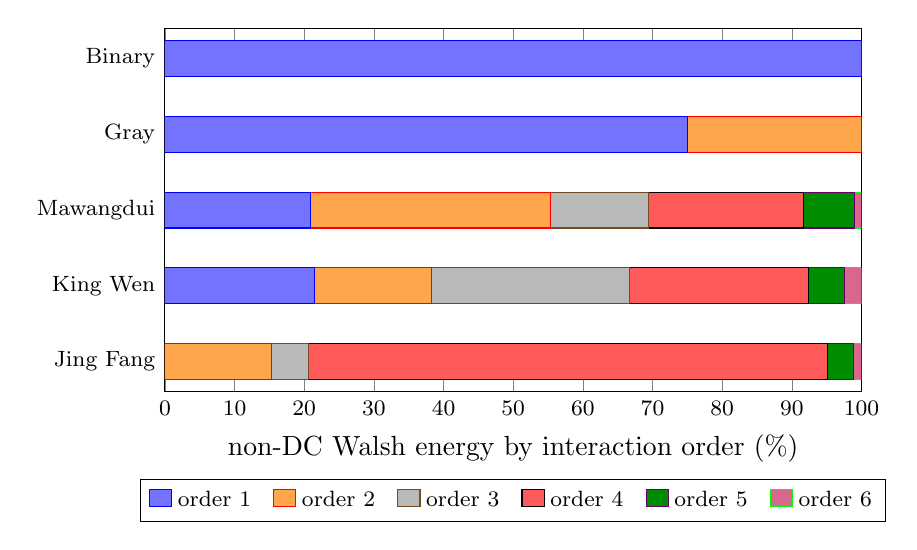
\begin{tikzpicture}
\begin{axis}[
  xbar stacked, width=0.86\textwidth, height=6.2cm,
  xmin=0, xmax=100,
  xlabel={non-DC Walsh energy by interaction order (\%)},
  ytick=data,
  symbolic y coords={Jing Fang,King Wen,Mawangdui,Gray,Binary},
  bar width=13pt,
  legend style={at={(0.5,-0.24)}, anchor=north, legend columns=6, font=\footnotesize, /tikz/every even column/.append style={column sep=6pt}},
  tick label style={font=\footnotesize},
]
\addplot+[fill=blue!55] coordinates {(100,Binary)(75,Gray)(20.9,Mawangdui)(21.5,King Wen)(0.0,Jing Fang)};
\addplot+[fill=orange!70] coordinates {(0,Binary)(25,Gray)(34.4,Mawangdui)(16.8,King Wen)(15.3,Jing Fang)};
\addplot+[fill=gray!55] coordinates {(0,Binary)(0,Gray)(14.1,Mawangdui)(28.4,King Wen)(5.3,Jing Fang)};
\addplot+[fill=red!65] coordinates {(0,Binary)(0,Gray)(22.3,Mawangdui)(25.7,King Wen)(74.5,Jing Fang)};
\addplot+[fill=green!55!black] coordinates {(0,Binary)(0,Gray)(7.3,Mawangdui)(5.1,King Wen)(3.8,Jing Fang)};
\addplot+[fill=purple!60] coordinates {(0,Binary)(0,Gray)(1.2,Mawangdui)(2.5,King Wen)(1.2,Jing Fang)};
\legend{order 1, order 2, order 3, order 4, order 5, order 6}
\end{axis}
\end{tikzpicture}
\caption{Walsh energy by interaction order for the five orderings (percent of non-DC energy). Binary is a pure first-order tone; Jing Fang is anti-linear, with 74.5 percent in fourth-order interactions and none in the first.}
\label{fig:fingerprints}
\end{figure}

Three observations. First, the binary and Gray orderings behave as calibration: the binary signal is exactly linear (all energy in order 1), and Gray is nearly so. Second, the Jing Fang arrangement is the anti-linear order: its signal contains no first-order component at all, and concentrates 74.5 percent of its energy in fourth-order interactions, a signature produced by the palace generation schedule (cumulative flips plus the two soul transformations); the loner of Section~\ref{sec:kinship} also has the strangest spectrum, and the fingerprint shows in what way. Third, the dominant cyclic harmonic of the King Wen signal is $k = 16$, that is period 4: the same scale as the yang-balanced groups of four reported by Chan (2026). Two independent instruments, a time-domain count and a Fourier decomposition, point to the same four-hexagram periodicity in the received sequence; we record the convergence without proposing a mechanism.

\section{Related work}

Formal analysis of the King Wen sequence begins, in the current wave, with Chan (2026), who characterizes the sequence against 100,000 free permutations and reports the four signatures re-analyzed in Section~\ref{sec:pairs}, alongside uniformly negative results on their utility for neural network training; and Radisic (2026), who settles the pairing question with a Lean-verified optimality theorem. Our contribution is orthogonal to both: comparative permutation statistics across the historical orderings, a conditional re-analysis, a mechanism for the inter-order kinship, and the orientation battery.

The comparative study of the orderings themselves has a philological literature: Shaughnessy (1996) reconstructs and translates the Mawangdui manuscript, Shaughnessy (2014) situates it among the recently unearthed Changes manuscripts, and Han Zhongmin's study of the silk-manuscript hexagram sequence offers a qualitative comparison with the received order. The trigram-family doctrine underlying Section~\ref{sec:kinship} and the Eight Palaces construction are documented in Nielsen (2003). The binary reading of the diagrams and its history run through Leibniz (1703) and Ryan (1996). Earlier quantitative observations exist outside the academic literature: the even/odd profile of first-order differences was tabulated by McKenna in the 1980s within an interpretive framework we do not adopt; an independently published proposal that nuclear hexagrams decide pair orientation is tested, and not confirmed in its simple form, in Section~\ref{sec:pairs}; and the cycle type $[52, 10, 2]$ of the King Wen permutation relative to binary order, noted on an independent mathematics website, reproduces under our conventions. The tradition's own account of the sequence, the Xugua commentary, is narrative and is not treated here as a structural hypothesis.

\section{Reproducibility}

The primary artifact accompanying this paper is a self-contained replication package:

\begin{center}
\url{https://github.com/theoriginaliching/kingwen-orderings-replication}\\[0.3em]
\url{https://paper.theoriginaliching.com}
\end{center}

\noindent
(the repository is the primary artifact; the second address is a human-readable gateway to the same package. Archived version: DOI pending). It contains the manuscript source, the compiled PDF and a single script, \texttt{verify\_paper.py}, which reproduces every numerical claim made here from first principles, using only the Python standard library, with no network access and no data files. The only external datum is the received King Wen sequence, embedded as a literal table; every other ordering is generated from the construction rules given in Section~2, so the package verifies the constructions as well as the statistics. It prints one line per check, showing the reproduced value beside the value printed in this paper, and exits zero if and only if all of them pass:

\begin{center}
\texttt{python3 verify\_paper.py} \qquad \texttt{tectonic paper.tex}
\end{center}

As a secondary resource, the same material is explored in an extended interactive laboratory of 44 experiments at \url{https://experiments.theoriginaliching.com} (in Spanish; an English version is in progress), whose assertion suite comprises 61 sections executed as a publication gate (exit status zero required); computed statistics are frozen as assertions once verified, so that no figure can drift silently.

Throughout the project, a dual-derivation protocol was followed: each result was implemented at least twice, independently and with different random seeds, before publication. The protocol is not ceremonial; it caught and corrected errors in both directions during development, including an early correction of the palace generation order against the documented bagong sequence, a sampling-length error in one of our own preliminary $p$-values, and the discrepancy reported in Section~\ref{sec:pairs}. Monte Carlo results in this paper state their sample sizes and seeds; percentile conventions on integer statistics are declared where they matter.

\section{Scope and limitations}

This paper makes claims about orderings as combinatorial objects, and only those. It makes no numerological claims: readings that attach the golden ratio to the King Wen sequence, quantum mechanics to the oracle, or market behavior to the hexagrams fall outside its subject and, in our assessment, outside demonstrability. Three limitations are intrinsic. First, the King Wen sequence is a single fixed object; analyses of its internal structure (Sections 5.4 to 5.6) face a sample size that will never grow, and we have stated the resulting limit of demonstrability explicitly. Second, the interpretation of the family gradient as a shared convention (Section 4.3) is historical framing for a statistical finding; the direction of influence between the orderings, or from a common source, is not established here. Third, signal-based results (Section~\ref{sec:spectral}) depend on declared encoding conventions; rank-based results (Sections 3 to 5) do not.

\section{Conclusion}

Measured against binary counting, the three historical orderings of the hexagrams are uncorrelated with binary counting: two of them exactly at the null expectation, the third consistent with zero. Measured against one another, the two oldest recognize each other: not through their pairs, which Mawangdui's octets actively separate, but through a shared gradient of trigram families that the manuscript makes explicit and the received sequence carries as a tendency. And measured against its own last open question, the King Wen sequence yields one coherent candidate rule, the doctrine of correct centers, standing exactly at the boundary where twenty-eight pairs of evidence stop being able to decide. Three millennia asked what principle orders the Book of Changes. Part of the answer, it turns out, is a precise description of where the answer must end.

\section*{Acknowledgments}

The verification suite, exploratory computations and a first draft of this manuscript were prepared with the assistance of an AI system (Anthropic's Claude). Every numerical claim was independently re-derived and is asserted by the automated test suite described in Section~8; the author takes full responsibility for the content.

\begin{thebibliography}{9}
% Author-date; all entries verified online during the project except where flagged.
% Flagged entries must be completed before submission; nothing is cited from memory.

\bibitem{chan2026} Chan, A. (2026). Statistical properties of the King Wen sequence: An anti-habituation structure that does not improve neural network training [Preprint]. arXiv. \url{https://arxiv.org/abs/2604.09234}

\bibitem{hon2023} Hon, T. (2023). Chinese philosophy of change (Yijing). In E. N. Zalta \& U. Nodelman (Eds.), \textit{The Stanford Encyclopedia of Philosophy}. \url{https://plato.stanford.edu/entries/chinese-change/}

\bibitem{leibniz1703} Leibniz, G. W. (1703). Explication de l'arithmétique binaire. \textit{Mémoires de l'Académie Royale des Sciences}, année 1703.

\bibitem{nielsen2003} Nielsen, B. (2003). \textit{A companion to Yi jing numerology and cosmology: Chinese studies of images and numbers from Han (202 BCE--220 CE) to Song (960--1279 CE)}. RoutledgeCurzon.

\bibitem{radisic2026} Radisic, A. (2026). Optimal equivariant matchings on the 6-cube: With an application to the King Wen sequence [Preprint]. arXiv. \url{https://arxiv.org/abs/2601.07175}

\bibitem{ryan1996} Ryan, J. A. (1996). Leibniz' binary system and Shao Yong's ``Yijing''. \textit{Philosophy East and West, 46}(1), 59--90. \url{https://doi.org/10.2307/1399337}

\bibitem{shaughnessy1996} Shaughnessy, E. L. (1996). \textit{I Ching: The classic of changes: The first English translation of the newly discovered second-century B.C. Mawangdui texts}. Ballantine Books.

\bibitem{shaughnessy2014} Shaughnessy, E. L. (2014). \textit{Unearthing the changes: Recently discovered manuscripts of the Yi jing (I ching) and related texts}. Columbia University Press.

% Nota resuelta: el estudio de Han Zhongmin sobre la secuencia del manuscrito de seda se menciona
% descriptivamente en la Seccion 7; no fue posible verificar en linea una ficha bibliografica
% completa, asi que no lleva entrada formal, conforme a la regla del proyecto de no citar de memoria.
% [DECISION DE ESTILO] McKenna y la propuesta nuclear: ambas son fuentes web sin ficha academica;
% se mencionan en el cuerpo como "outside the academic literature" sin entrada bibliografica formal.

\end{thebibliography}

\end{document}
